\documentclass[11pt,a4paper]{article}
\usepackage[margin=22mm]{geometry}
\usepackage[T1]{fontenc}
\usepackage{lmodern,amsmath,amssymb,booktabs,tikz,enumitem}
\usetikzlibrary{arrows.meta,positioning}
\usepackage[colorlinks=true,urlcolor=blue]{hyperref}
\definecolor{zero}{HTML}{0072B2}
\definecolor{one}{HTML}{D55E00}
\definecolor{muted}{HTML}{65717B}
\definecolor{pale}{HTML}{EEF4F8}
\setlength{\parindent}{0pt}
\setlength{\parskip}{6pt}
\setlist{nosep,leftmargin=*}
\tikzset{stzero/.style={circle,draw=zero,fill=white,thick,minimum size=6mm,inner sep=1pt,text=zero},
 o/.style={circle,draw=one,fill=one,minimum size=6mm,inner sep=1pt,text=white},
 lin/.style={very thick,zero,-{Stealth[length=2mm]}},
 lost/.style={thick,muted,dashed,-{Stealth[length=2mm]}},
 lab/.style={font=\small,align=left}}
\newcommand{\head}[2]{\noindent{\small\sffamily\color{muted}BISSE / #1}\par
 {\LARGE\sffamily\bfseries #2}\par\vspace{3mm}}
\begin{document}
\head{01 / THE PROCESS}{Two states, four possibilities}
BiSSE couples a binary character (0 or 1) to speciation and extinction.
This note redraws the supplied sketch and derives the backward likelihood equations.
\textbf{Speciation itself does not change the state:} both daughters inherit
their parent's state. State changes occur along lineages.

\begin{center}
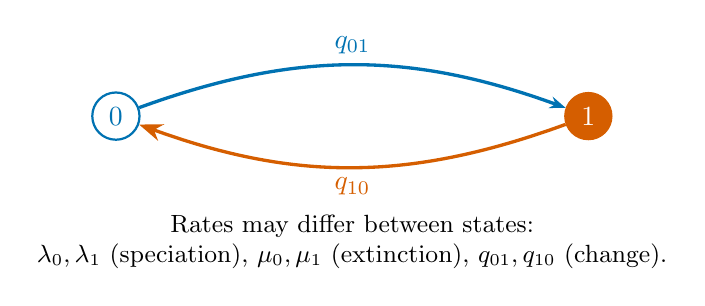
\begin{tikzpicture}[x=1cm,y=1cm]
\node[stzero] (a) at (0,0) {0}; \node[o] (b) at (6,0) {1};
\draw[lin,bend left=20] (a) to node[above] {$q_{01}$} (b);
\draw[very thick,one,-{Stealth},bend left=20] (b) to node[below] {$q_{10}$} (a);
\node[lab,align=center] at (3,-1.6) {Rates may differ between states:\\
 $\lambda_0,\lambda_1$ (speciation), $\mu_0,\mu_1$ (extinction), $q_{01},q_{10}$ (change).};
\end{tikzpicture}
\end{center}

For a lineage in state 0, define \(r_0=\lambda_0+\mu_0+q_{01}\).
Over a short forward-time interval \(\Delta t\), the alternatives are:
\begin{center}
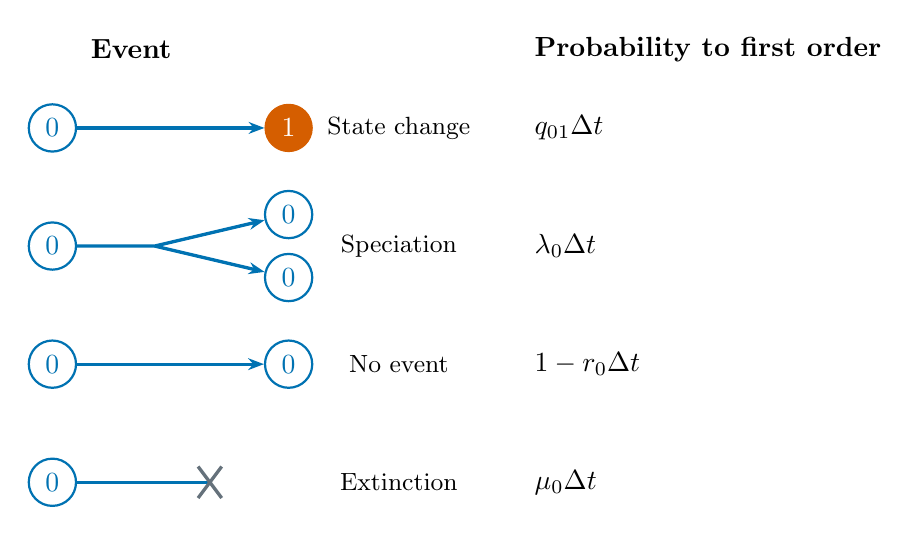
\begin{tikzpicture}[x=1cm,y=1cm]
\node[lab,font=\bfseries] at (1,0) {Event};
\node[lab,font=\bfseries,anchor=west] at (6,0) {Probability to first order};
\node[stzero] (a1) at (0,-1) {0}; \node[o] (b1) at (3,-1) {1};
\draw[lin] (a1)--(b1); \node[lab] at (4.4,-1) {State change};
\node[anchor=west] at (6,-1) {$q_{01}\Delta t$};
\node[stzero] (a2) at (0,-2.5) {0}; \node[stzero] (b2) at (3,-2.1) {0};
\node[stzero] (c2) at (3,-2.9) {0};
\draw[lin] (a2)--(1.3,-2.5)--(b2); \draw[lin] (1.3,-2.5)--(c2);
\node[lab] at (4.4,-2.5) {Speciation}; \node[anchor=west] at (6,-2.5) {$\lambda_0\Delta t$};
\node[stzero] (a3) at (0,-4) {0}; \node[stzero] (b3) at (3,-4) {0};
\draw[lin] (a3)--(b3); \node[lab] at (4.4,-4) {No event};
\node[anchor=west] at (6,-4) {$1-r_0\Delta t$};
\node[stzero] (a4) at (0,-5.5) {0}; \draw[lin,-] (a4)--(2,-5.5);
\draw[very thick,muted] (1.85,-5.7)--(2.15,-5.3) (1.85,-5.3)--(2.15,-5.7);
\node[lab] at (4.4,-5.5) {Extinction}; \node[anchor=west] at (6,-5.5) {$\mu_0\Delta t$};
\end{tikzpicture}
\end{center}
Terms of order \(o(\Delta t)\) are omitted; two or more events have negligible
probability to first order. The exact no-event probability for constant rates is
\(e^{-r_0\Delta t}\). A no-event outcome is \emph{not} extinction.

\subsection*{Our clock: age before the present}
\begin{center}
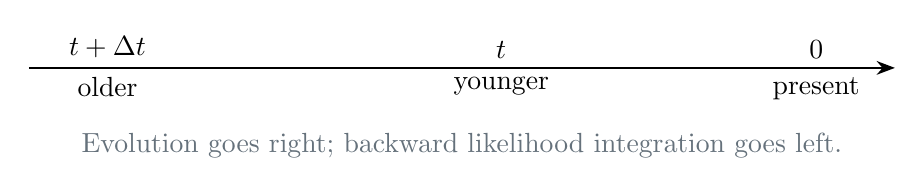
\begin{tikzpicture}[x=1cm]
\draw[-{Stealth},thick] (0,0)--(11,0);
\node[above] at (1,0) {$t+\Delta t$}; \node[above] at (6,0) {$t$};
\node[above] at (10,0) {$0$};
\node[below] at (1,0) {older}; \node[below] at (6,0) {younger};
\node[below] at (10,0) {present};
\node[below,muted] at (5.5,-.7) {Evolution goes right; backward likelihood integration goes left.};
\end{tikzpicture}
\end{center}

\newpage
\head{02 / OBSERVED DESCENDANTS}{Deriving the equation for $D_0$}
\(D_i(t)\) is the likelihood of the observed descendant subtree and its tip
states, given a lineage in state \(i\) at age \(t\).
\(E_i(t)\) is the probability of leaving \emph{no living descendants} today.
Here we assume complete sampling of living species.

At age \(t\), the values \(D_0,D_1,E_0,E_1\) are already known from the
younger part of the tree. To obtain \(D_0(t+\Delta t)\), sum all compatible
ways to cross the short interval starting in state 0.

\begin{center}
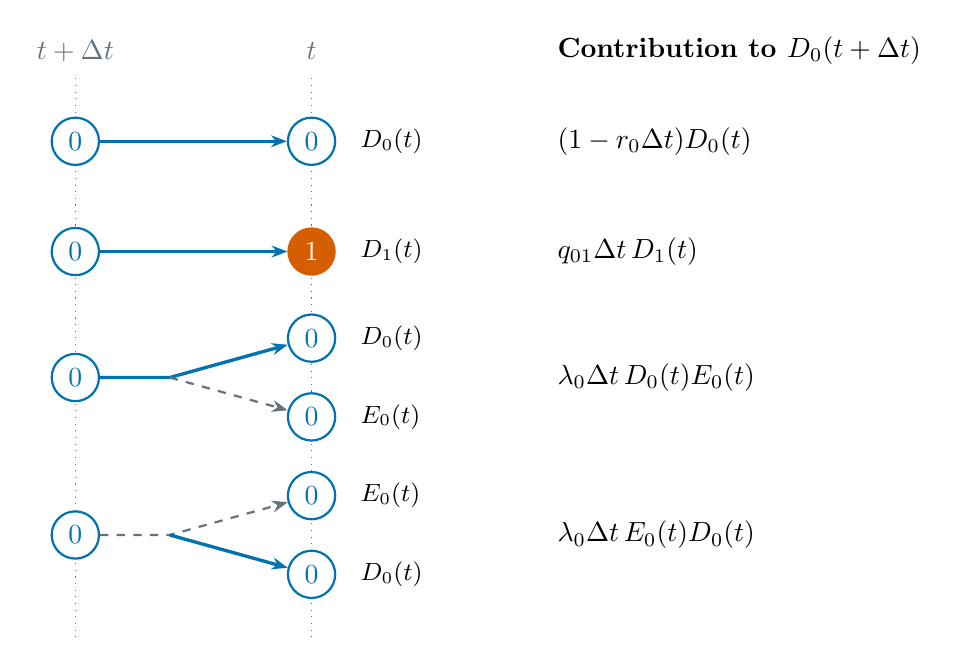
\begin{tikzpicture}[x=1cm,y=1cm]
\node[muted] at (0,.45) {$t+\Delta t$}; \node[muted] at (3,.45) {$t$};
\node[anchor=west,font=\bfseries] at (6,.45) {Contribution to $D_0(t+\Delta t)$};
\draw[muted,dotted] (0,.1)--(0,-7); \draw[muted,dotted] (3,.1)--(3,-7);
\node[stzero] (a) at (0,-.7) {0}; \node[stzero] (b) at (3,-.7) {0}; \draw[lin] (a)--(b);
\node[lab,anchor=west] at (3.5,-.7) {$D_0(t)$};
\node[anchor=west] at (6,-.7) {$(1-r_0\Delta t)D_0(t)$};
\node[stzero] (a) at (0,-2.1) {0}; \node[o] (b) at (3,-2.1) {1}; \draw[lin] (a)--(b);
\node[lab,anchor=west] at (3.5,-2.1) {$D_1(t)$};
\node[anchor=west] at (6,-2.1) {$q_{01}\Delta t\,D_1(t)$};
\node[stzero] (a) at (0,-3.7) {0}; \node[stzero] (b) at (3,-3.2) {0}; \node[stzero] (c) at (3,-4.2) {0};
\draw[lin] (a)--(1.2,-3.7)--(b); \draw[lost] (1.2,-3.7)--(c);
\node[lab,anchor=west] at (3.5,-3.2) {$D_0(t)$}; \node[lab,anchor=west] at (3.5,-4.2) {$E_0(t)$};
\node[anchor=west] at (6,-3.7) {$\lambda_0\Delta t\,D_0(t)E_0(t)$};
\node[stzero] (a) at (0,-5.7) {0}; \node[stzero] (b) at (3,-5.2) {0}; \node[stzero] (c) at (3,-6.2) {0};
\draw[lost] (a)--(1.2,-5.7)--(b); \draw[lin] (1.2,-5.7)--(c);
\node[lab,anchor=west] at (3.5,-5.2) {$E_0(t)$}; \node[lab,anchor=west] at (3.5,-6.2) {$D_0(t)$};
\node[anchor=west] at (6,-5.7) {$\lambda_0\Delta t\,E_0(t)D_0(t)$};
\end{tikzpicture}
\end{center}
Solid paths carry the observed descendants. Dashed paths must leave no living
descendants: they need not die \emph{inside} this short interval.
Immediate death contributes \(\mu_0\Delta t\times0\): it cannot produce the
nonempty observed subtree.

\begin{align*}
D_0(t+\Delta t)={}&(1-r_0\Delta t)D_0(t)+q_{01}\Delta t D_1(t)\\
&+2\lambda_0\Delta t D_0(t)E_0(t)+o(\Delta t).
\end{align*}
Subtract \(D_0(t)\), divide by \(\Delta t\), and take the limit:
\[
\boxed{\frac{dD_0}{dt}=-(\lambda_0+\mu_0+q_{01})D_0
                         +q_{01}D_1+2\lambda_0D_0E_0.}
\]
\textbf{Why two?} Either daughter can carry the observed subtree while the
other disappears. These are two distinct possibilities, even though both
daughters initially have state 0. Two surviving daughters would create an
observed branching node, not a hidden event along this branch.

\newpage
\head{03 / NO LIVING DESCENDANTS}{Deriving the equation for $E_0$}
Now the required outcome is different: \emph{the entire descendant clade must
be extinct at the present}. The same short-interval reasoning gives:

\begin{center}
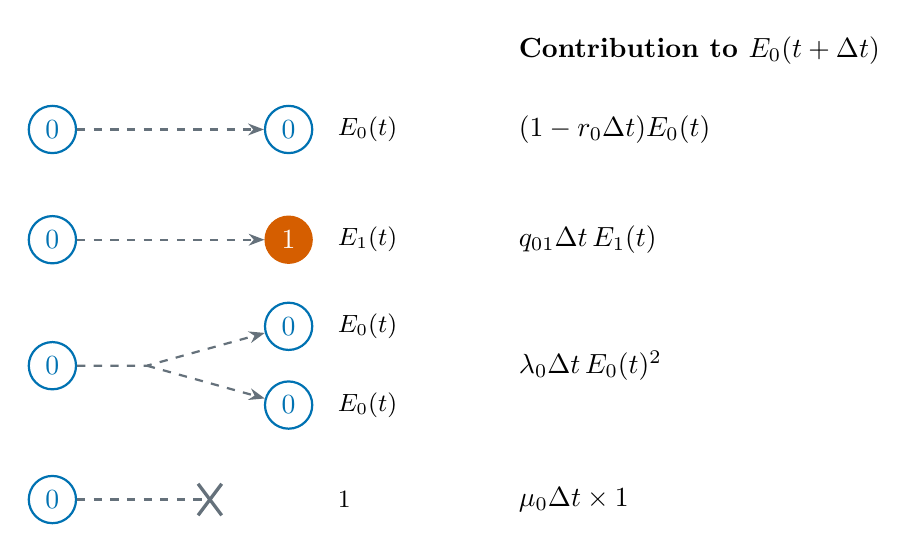
\begin{tikzpicture}[x=1cm,y=1cm]
\node[anchor=west,font=\bfseries] at (5.8,0) {Contribution to $E_0(t+\Delta t)$};
\node[stzero] (a) at (0,-1) {0}; \node[stzero] (b) at (3,-1) {0}; \draw[lost] (a)--(b);
\node[lab,anchor=west] at (3.5,-1) {$E_0(t)$};
\node[anchor=west] at (5.8,-1) {$(1-r_0\Delta t)E_0(t)$};
\node[stzero] (a) at (0,-2.4) {0}; \node[o] (b) at (3,-2.4) {1}; \draw[lost] (a)--(b);
\node[lab,anchor=west] at (3.5,-2.4) {$E_1(t)$};
\node[anchor=west] at (5.8,-2.4) {$q_{01}\Delta t\,E_1(t)$};
\node[stzero] (a) at (0,-4) {0}; \node[stzero] (b) at (3,-3.5) {0}; \node[stzero] (c) at (3,-4.5) {0};
\draw[lost] (a)--(1.2,-4)--(b); \draw[lost] (1.2,-4)--(c);
\node[lab,anchor=west] at (3.5,-3.5) {$E_0(t)$}; \node[lab,anchor=west] at (3.5,-4.5) {$E_0(t)$};
\node[anchor=west] at (5.8,-4) {$\lambda_0\Delta t\,E_0(t)^2$};
\node[stzero] (a) at (0,-5.7) {0}; \draw[lost,-] (a)--(2,-5.7);
\draw[very thick,muted] (1.85,-5.9)--(2.15,-5.5) (1.85,-5.5)--(2.15,-5.9);
\node[lab,anchor=west] at (3.5,-5.7) {$1$};
\node[anchor=west] at (5.8,-5.7) {$\mu_0\Delta t\times1$};
\end{tikzpicture}
\end{center}
Immediate death guarantees the required outcome, so its remaining probability
is 1. After speciation, \emph{both} daughters must die out. Their futures are
independent conditional on their states, producing \(E_0^2\).
There is no factor of two: exchanging two extinct daughters is not a new outcome.
\begin{align*}
E_0(t+\Delta t)={}&(1-r_0\Delta t)E_0(t)+q_{01}\Delta t E_1(t)\\
&+\lambda_0\Delta t E_0(t)^2+\mu_0\Delta t+o(\Delta t),
\end{align*}
\[
\boxed{\frac{dE_0}{dt}=\mu_0-(\lambda_0+\mu_0+q_{01})E_0
                         +q_{01}E_1+\lambda_0 E_0^2.}
\]

\subsection*{The complete backward system}
Let \(r_1=\lambda_1+\mu_1+q_{10}\). All quantities on the right are evaluated at \(t\):
\[
\begin{aligned}
\dot E_0&=\mu_0-r_0E_0+q_{01}E_1+\lambda_0E_0^2,\\
\dot E_1&=\mu_1-r_1E_1+q_{10}E_0+\lambda_1E_1^2,\\
\dot D_0&=-r_0D_0+q_{01}D_1+2\lambda_0E_0D_0,\\
\dot D_1&=-r_1D_1+q_{10}D_0+2\lambda_1E_1D_1.
\end{aligned}
\]
These are derivatives with respect to \emph{increasing age}: integrate from
the tips into the past. The equations agree with
\texttt{diversitree:::derivs.bisse} (checked for this note).

\newpage
\head{04 / FROM LIKELIHOODS TO MAPS}{Tips, nodes and forward simulation}
\subsection*{1. Start at the observed tips}
For a known state-0 tip and complete sampling,
\[
\mathbf D(0)=\begin{pmatrix}1\\0\end{pmatrix},\qquad
\mathbf E(0)=\begin{pmatrix}0\\0\end{pmatrix}.
\]
A state-1 tip instead has \(\mathbf D(0)=(0,1)^{\mathsf T}\).
An extant lineage cannot already have no living descendants, hence \(E_i(0)=0\).
The \(E\) curves are shared across branches; \(D\) depends on each branch's
observed descendants. \(D_0+D_1\) need not equal 1.

\subsection*{2. Combine descendants at an observed node}
\begin{center}
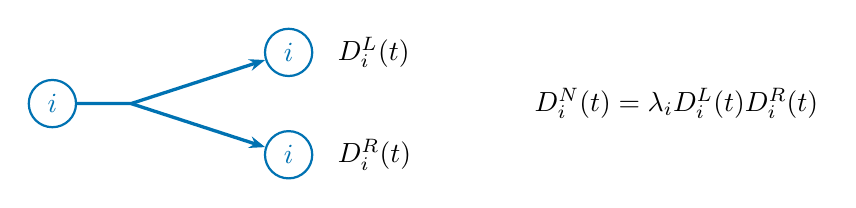
\begin{tikzpicture}[x=1cm,y=1cm]
\node[stzero] (p) at (0,0) {$i$}; \node[stzero] (l) at (3,.65) {$i$}; \node[stzero] (r) at (3,-.65) {$i$};
\draw[lin] (p)--(1,0)--(l); \draw[lin] (1,0)--(r);
\node[anchor=west] at (3.5,.65) {$D_i^L(t)$};
\node[anchor=west] at (3.5,-.65) {$D_i^R(t)$};
\node[anchor=west] at (6,0) {$D_i^N(t)=\lambda_iD_i^L(t)D_i^R(t)$};
\end{tikzpicture}
\end{center}
Here both daughters are observed. There is no hidden-side factor \(2E_i\).
The two node likelihoods become the boundary values for the older incoming
branch. Before additional survival conditioning, the root likelihood is
\(L=\pi_0D_0^{\rm root}+\pi_1D_1^{\rm root}\), with any numerical scaling restored.

\subsection*{3. Use likelihoods to guide a forward history}
For a backbone lineage currently in state 0 at age \(t\), conditional event
rates at that age are
\[
\begin{array}{ll}
\text{State change }0\to1:&q_{01}D_1(t)/D_0(t),\\[2pt]
\text{Hidden split }0\to0+0:&2\lambda_0E_0(t),\\[2pt]
\text{Backbone death}:&0.
\end{array}
\]
These require \(D_0(t)>0\). Given that an event happens, normalize these rates
to choose its type. At a hidden split, either state-0 daughter can carry the
observed descendants; the other is simulated conditional on extinction.

\textbf{Timing must also be conditioned.} For constant original rates, the
probability of no event from age \(t\) down to \(u<t\) is
\[
S_i(t,u)=e^{-r_i(t-u)}\frac{D_i(u)}{D_i(t)}.
\]
Draw \(Z\sim\mathrm{Exp}(1)\) and solve \(-\log S_i(t,u)=Z\), unless the
branch endpoint is reached first. On an extinction-conditioned side lineage,
replace \(D\) with \(E\); its event weights are
\(\mu_i,\ q_{ij}E_j,\ \lambda_iE_i^2\).

\subsection*{Scope and reference}
This is standard BiSSE, not cladogenetic state change (ClaSSE).
With sampling fractions \(\rho_i<1\), \(E_i(0)=1-\rho_i\) means
\emph{no sampled descendants}, not necessarily extinction, and an observed
state-\(i\) tip has \(D_i(0)=\rho_i\).
No fossil observations are included here.

{\small Maddison, W. P., Midford, P. E. and Otto, S. P. (2007).
Estimating a binary character's effect on speciation and extinction.
\emph{Systematic Biology} 56:701--710.
\href{https://doi.org/10.1080/10635150701607033}{doi:10.1080/10635150701607033}.}
\end{document}
